\begin{figure}[H]
\centering
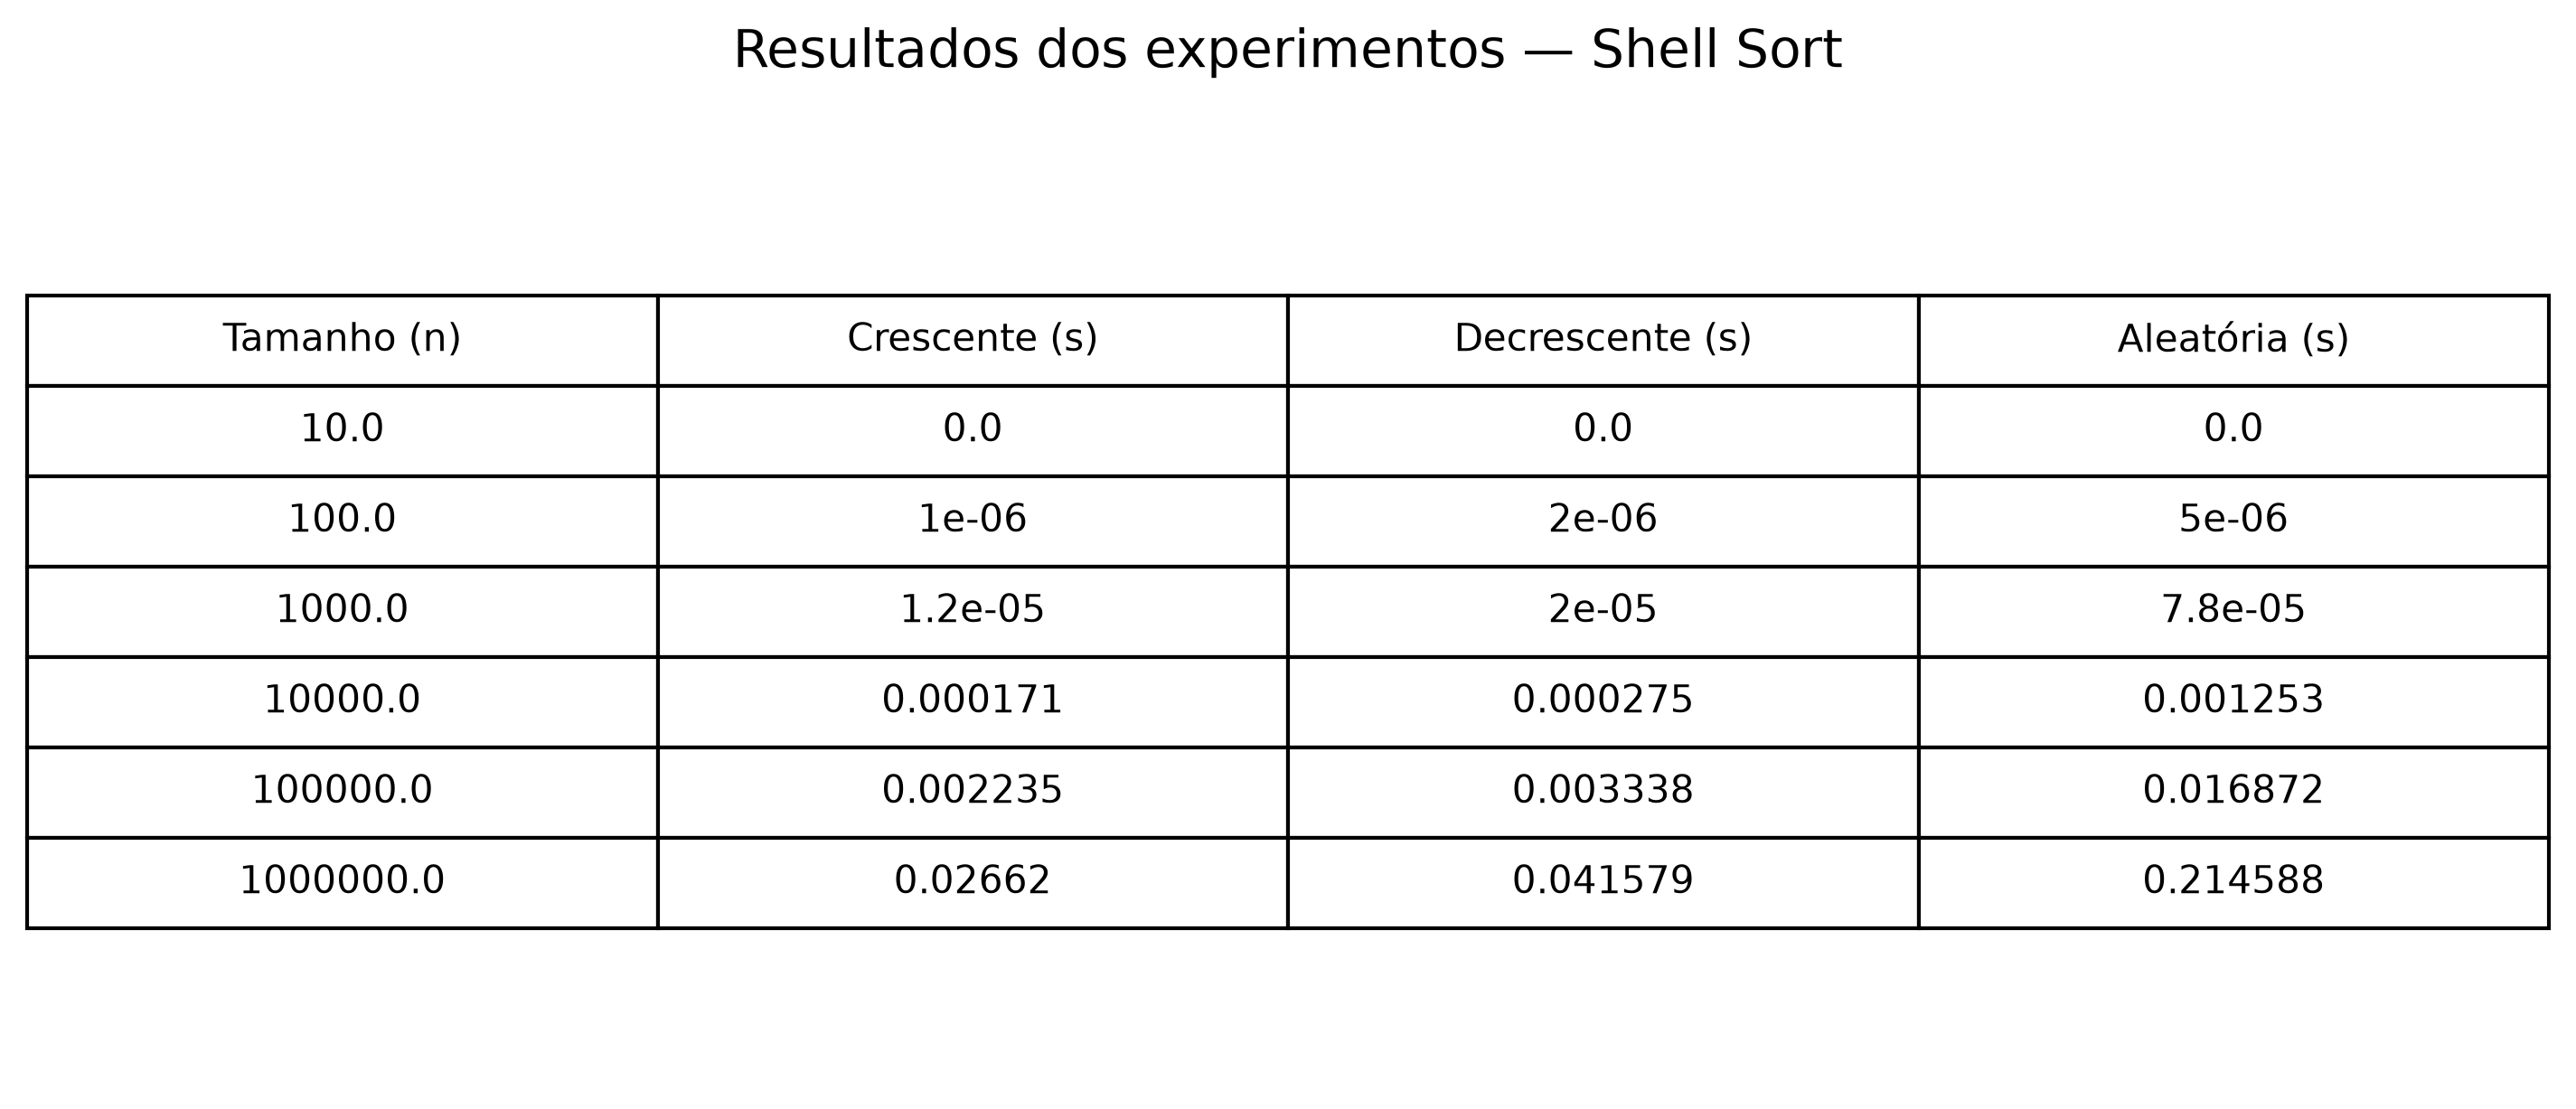
\includegraphics[width=16cm]{Imagens/Shell_Sort/tabela.png}
\caption{Tabela de tempo de execução do algoritmo Shell Sort}
\label{fig:tabela-shell}
\end{figure}

\begin{figure}[H]
\centering
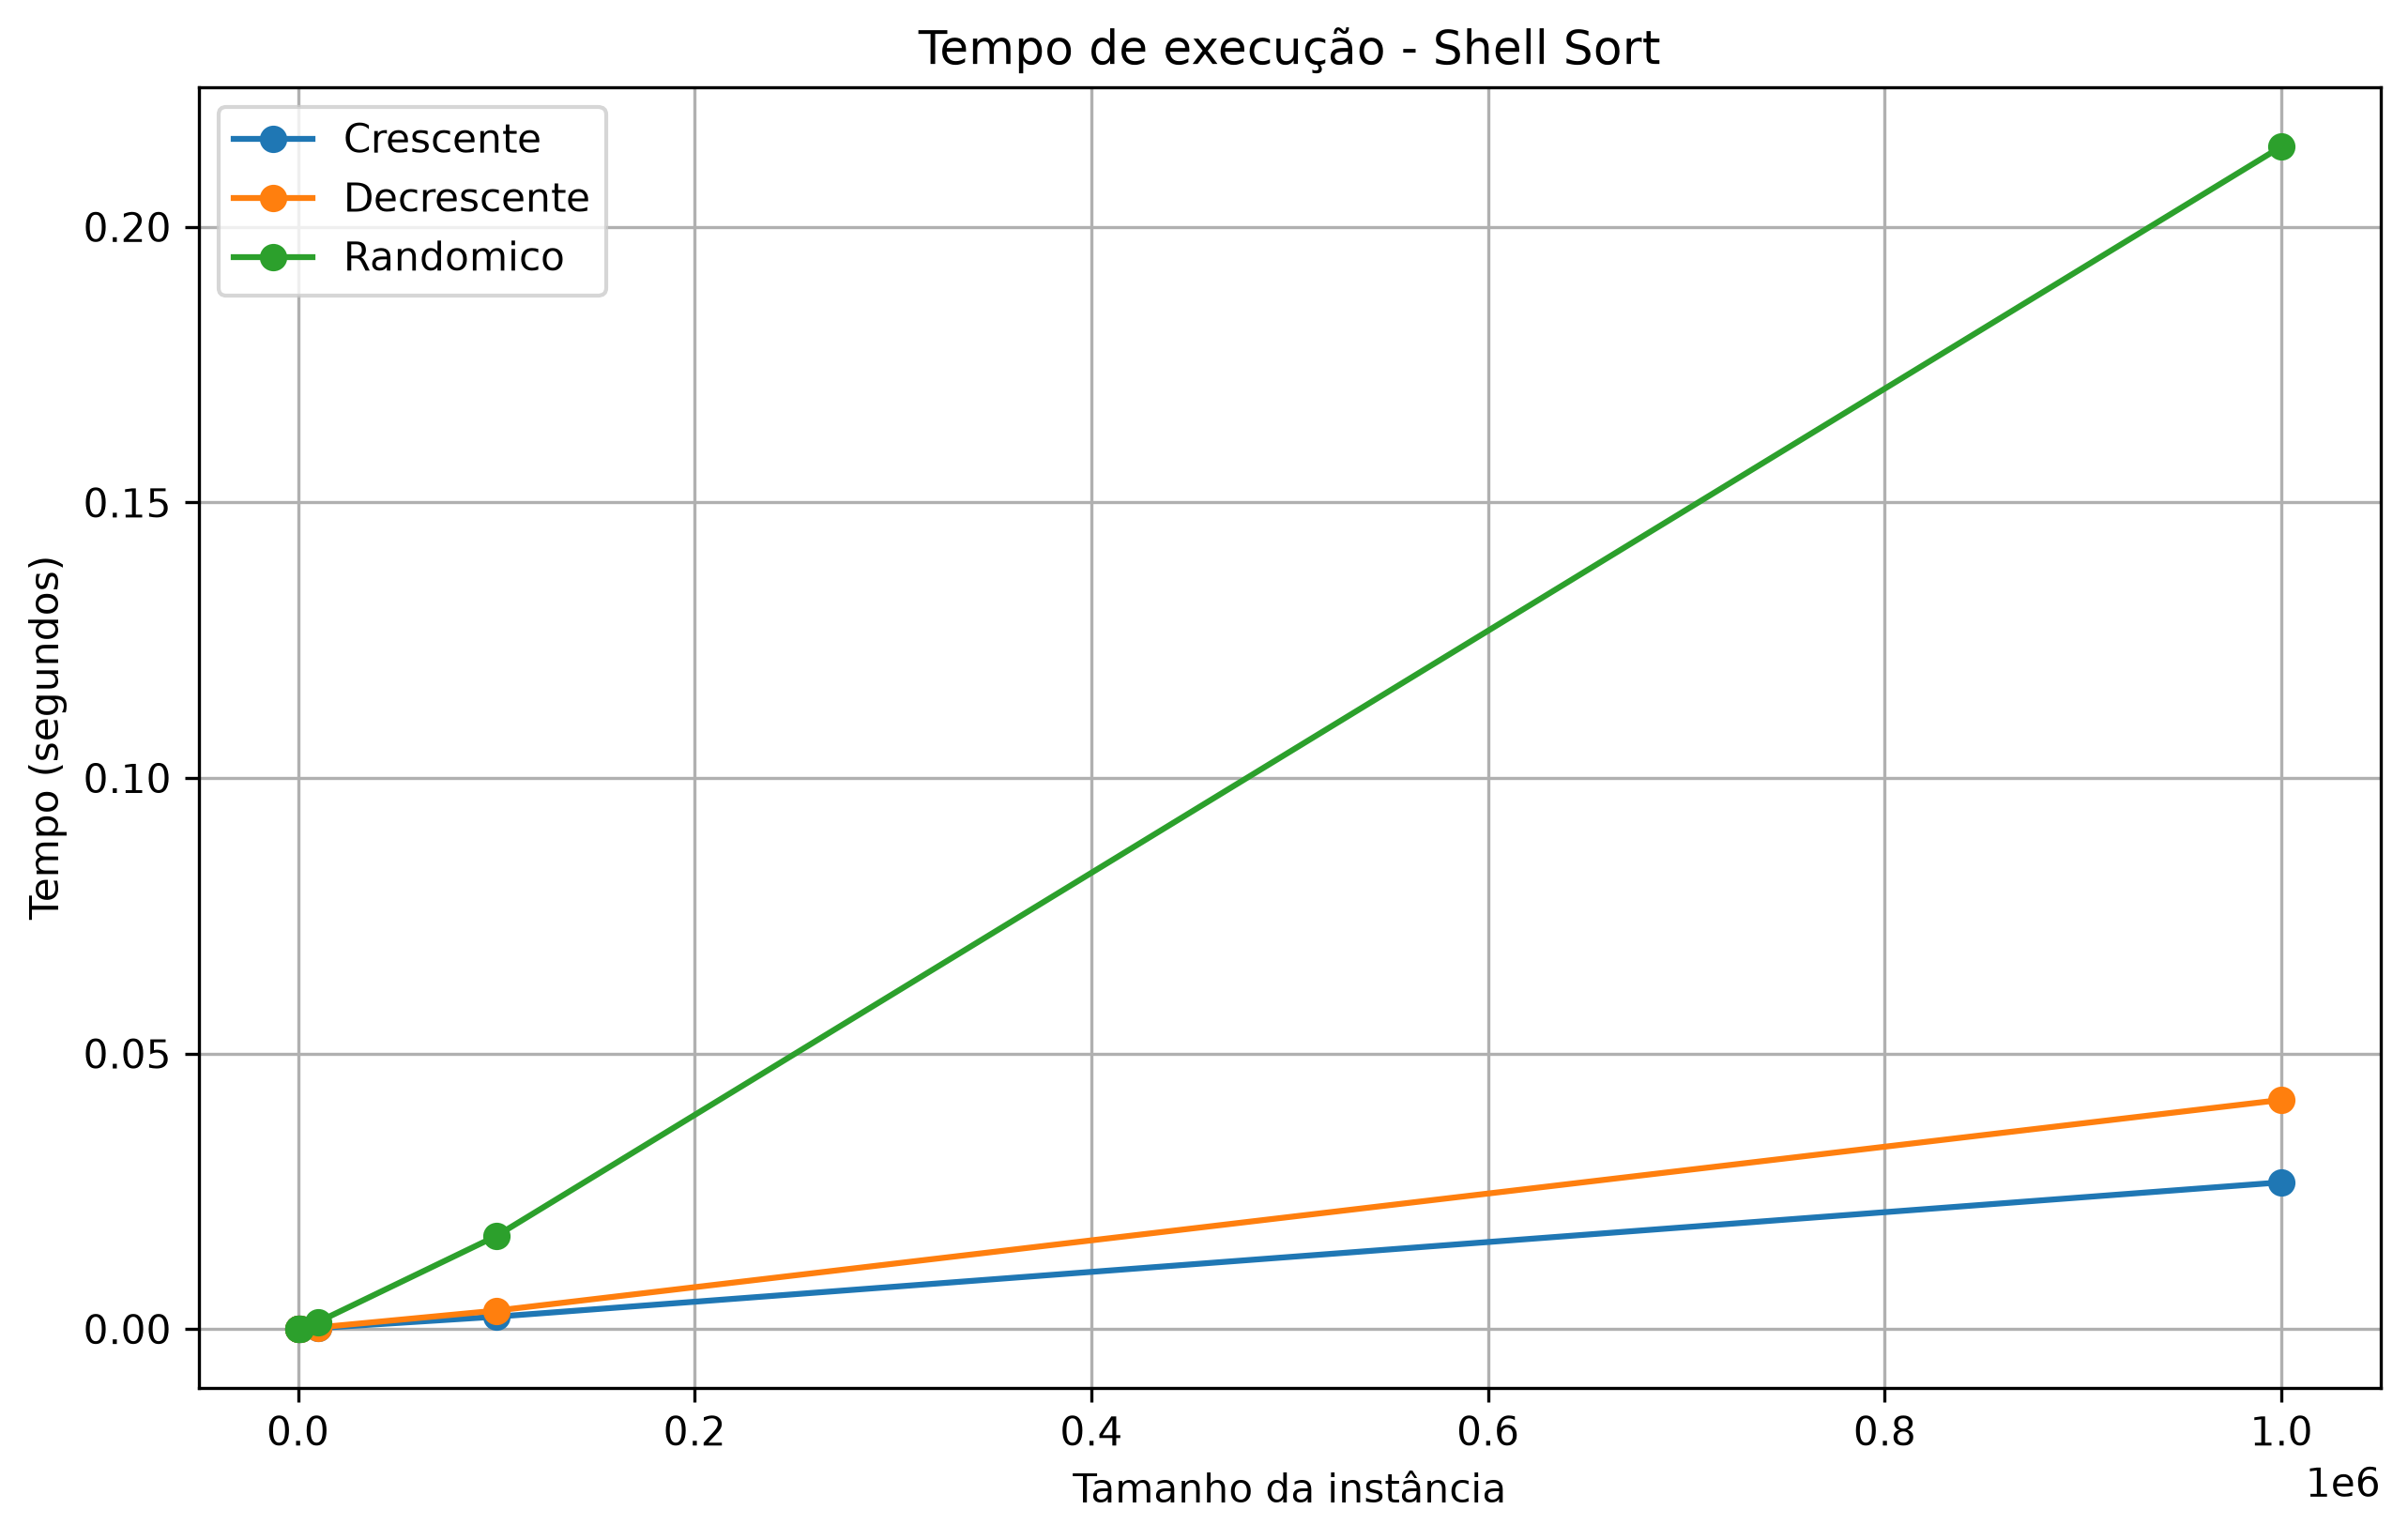
\includegraphics[width=10cm]{Imagens/Shell_Sort/grafico.png}
\caption{Gráfico de tempo de execução do algoritmo Shell Sort}
\label{fig:grafico-shell}
\end{figure}

Os resultados obtidos nos experimentos estão apresentados na tabela e no
gráfico. O algoritmo Shell Sort apresenta um comportamento diferente dos
demais algoritmos analisados, pois seu desempenho é influenciado pela
sequência de \textit{gaps} utilizada. Nos experimentos deste trabalho,
foi utilizado o divisor 2, produzindo uma sequência de \textit{gaps}
obtida pela divisão sucessiva do tamanho da entrada por 2 até atingir o
valor 1.

Nas instâncias ordenadas de forma crescente, os elementos já se encontram
em suas posições relativas para os diferentes \textit{gaps}, reduzindo a
quantidade de deslocamentos necessários durante a execução.

Nas instâncias ordenadas de forma decrescente, são necessários mais
deslocamentos para reorganizar os elementos. Entretanto, os
\textit{gaps} maiores permitem que elementos que estão distantes sejam
movimentados antes da etapa final, reduzindo parte da desordem do vetor.

As instâncias aleatórias apresentam comportamento intermediário, pois a
quantidade de comparações e deslocamentos depende da disposição inicial
dos elementos. O uso dos diferentes \textit{gaps} permite realizar
movimentações entre elementos distantes antes da ordenação final com
\textit{gap} igual a 1.

A partir dos dados, também é possível observar a influência do aumento do
tamanho da entrada no tempo de execução. O crescimento observado pode ser
relacionado à análise teórica do algoritmo, que depende da sequência de
\textit{gaps} utilizada. Para a sequência adotada neste trabalho, o pior
caso apresenta comportamento de ordem $\Theta(n^2)$, enquanto o melhor
caso apresenta comportamento de ordem $\Theta(n\log n)$.

Os resultados experimentais permitem, portanto, relacionar o
comportamento observado na tabela e no gráfico com a estratégia utilizada
pelo Shell Sort e com a influência da sequência de \textit{gaps} em seu
desempenho.
